\section{Sistema Nervioso}

El sistema nervioso se estudia principalmente en dos partes, sistema nervioso periférico (SNP), y sistema nervioso central (SNC). SNC es donde nos enfocaremos, se compone principalmente por la medula espinal y el encéfalo. Es en el encéfalo donde se encuentra el cerebro, cerebelo, y el tallo encefálico.\cite{sistemaNervioso}   

\textbf{¿Qué es un nervio?}
Un nervio es una gran colección de axones empacados todos juntos en una especie de cable (fibra); pasan vasos sanguíneos por en medio de los nervios. Esto es de lo que está formado el sistema nervioso. Se originan desde la médula espinal o el encéfalo. %(31 pares de nervios raquídeos) o el encéfalo (12 pares de nervios craneales).

\textbf{¿Qué son los nervios?}
Los nervios son estructuras conductoras de impulsos nerviosos, conformados por una colección de axones empacados en una especie de cable o, más específicamente, fibra. Todos los nervios, junto con sus axones, salen desde el cráneo o la médula espinal y cubren el resto del cuerpo.\cite{neurona_A_cerebro}


Estos pueden ser clasificados en:

\begin{itemize}
\item \textbf{Motores} salidas, ejecución/acción, se conectan y ejercen su acción sobre los músculos.
\item \textbf{Sensitivos} reciben señales de entrada, como en ojos, oídos y piel.
\item \textbf{Mixtos} son mayoría, tienen tanto fibras sensitivas como motoras.
\end{itemize}

Las ideas tomadas del SNC para el desarrollo de las RNA, son:
\begin{itemize}
 \item La serie de entradas, del mundo exterior hacia los nervios receptores.
 \item Una o varias salidas/respuestas ante un estímulo.
 \item Estructura de las conexiones entre los nervios motores, sensitivos, mixtos y el encéfalo o médula espinal. 
\end{itemize}

Entonces si vemos el SNC, solo como un sistema que nos permite sentir el mundo con el que interactuamos, a través de los nervios que están en nuestra piel. Y estos transmitir la información hasta nuestra médula espinal o cerebelo. Tenemos entonces la primera idea de una serie de entradas, que va a provocar de alguna forma, una o varias respuestas de nuestro cuerpo. Entonces es cuando se nota la existencia de una estructura que permite la conexión entre nuestros nervios y el encéfalo o médula espinal; esta estructura es la que da pie a las muchas formas de modelar una RNA.

\subsection{Cerebro}

Desde la parte tangible del cerebro hasta la intangible del pensamiento, esta directamente relacionada con la forma que funciona nuestro pensamiento y reacciones motoras.

El cerebro, por su gran tamaño, da lugar a un mejor registro de su actividad debido a la cantidad de sangre que se está bombeando continuamente. Se tienen identificadas regiones que se activan ante cierto estímulo.\cite{neurona_A_cerebro} Se detecta cuánta sangre se está bombeando en diferentes regiones del cerebro dependiendo de los estímulos que se le presentan a una persona; o si alguna persona tiene un padecimiento, se toman escaneos para ver qué regiones del cerebro están funcionando y cuáles presentan lesiones. A partir de las lesiones y de la identificación de la actividad que ya no se puede realizar de forma normal, se infiere qué región era responsable de esa actividad que ahora está dañada.\cite{estudiosF}

Para obtener más detalle de los estudios de la actividad del cerebro, ver el documental "The Brain with David Eagleman".

\subsection{Zonas funcionales}

En el cerebro, las diversas zonas indentificadas con funciones especificas, estan conectadas, por una ruta que se conoce como 
 ''la ruta desde la sensación hasta la cognición'' notemos un diagrama de la parte funcional del cerebro. \cite{sensAcogn}  


 \begin{figure}[h]
  \centering
  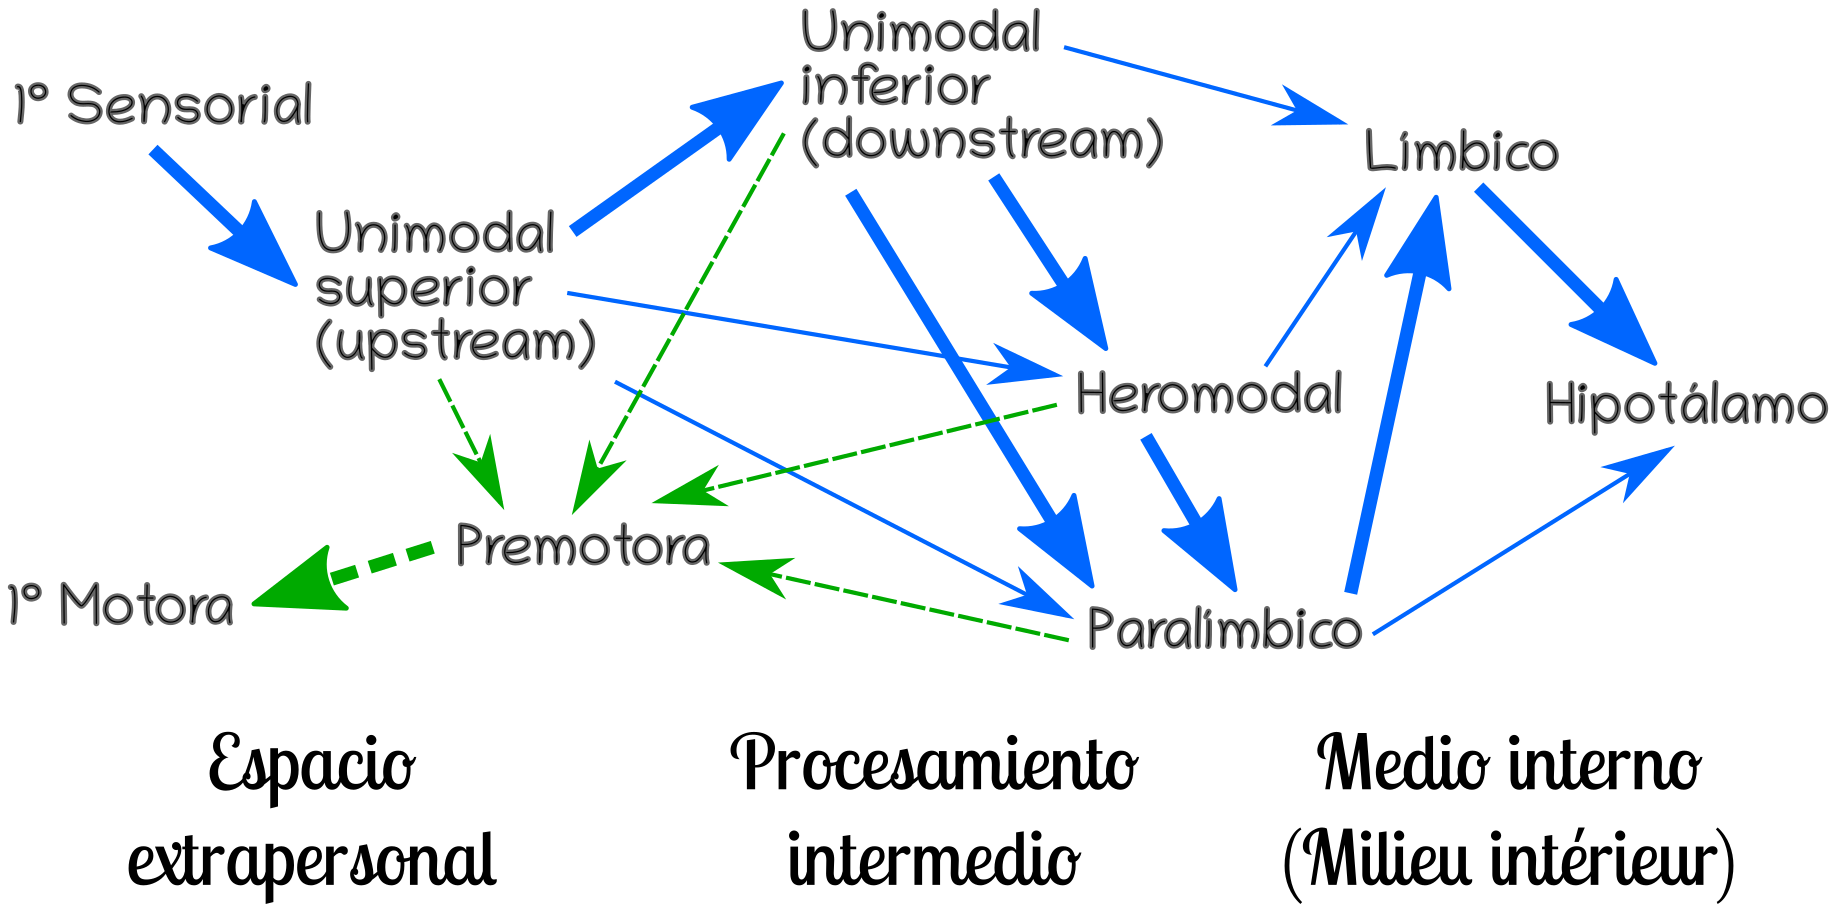
\includegraphics[width=0.9\textwidth]{../Figuras/zonasFuncionales.png}
  \caption{Diagrama de la arquitectura del cerebro a nivel funcional. \parencite{Mesulam1998}}
  \label{fig:zonasFun}
 \end{figure}

Explicación: en la primera parte (espacio extrapersonal) vamos a pensar en \textbf{la entrada sensorial}, que se enfoca en la visión o el audio (o demás sentidos). Su primera conexión es hacia la capa unimodal superior, donde se procesa la información de cada sentido de manera individual.

Luego están las capas intermedias (heromodal y demás), donde se dará un procesamiento intermedio; se juntarán varias características interpretadas por la primera capa, hacia varias neuronas encargadas de notar características más complejas.

Finalmente, llegamos al hipotálamo, que con todas las características dadas mandará a través de las capas intermedias una o varias respuestas, cuya etapa final se dará en la capa premotora, donde las neuronas de esta capa se comunican directamente con la \textbf{salida motora}.







